\section{Introduction}
\label{sec:intro}

\begin{figure}[!t]
    \centering
    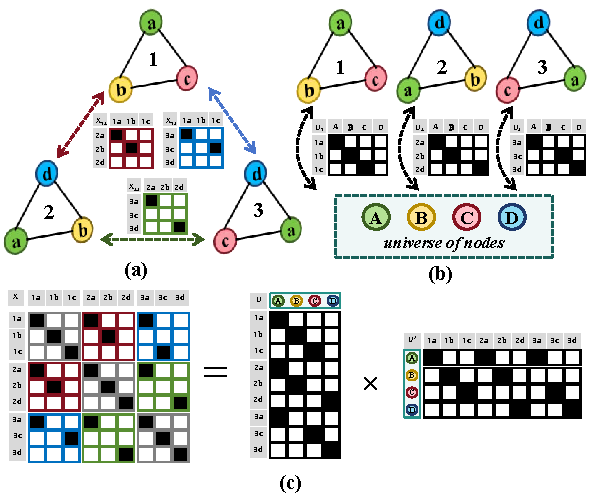
\includegraphics[width=0.98\linewidth]{Figures/motivation_.pdf}
    % \vspace{-10pt}
    \caption{Illustration of multi-graph matching using the \textit{universe of nodes}.
 (a) Direct pairwise matching between graphs 1, 2, and 3. (b) Multi-graph matching with the \textit{universe of nodes}. (c) Equivalence between (a) and (b) (see \textit{Lemma} 1 in Sec.~\ref{lemma1} for details).}
    \vspace{-10pt}
    \label{fig:moti}
\end{figure}

In the field of medical image processing, semantic segmentation is a technique that enables the precise identification and quantitative analysis of target regions. 
% This allows doctors to gain a clearer understanding of the spatial distribution of tumours, organs, and other important structures, thereby enhancing diagnostic accuracy, aiding in surgical planning, and facilitating the monitoring of disease progression.
% Currently, a considerable number of medical models can effectively perform segmentation tasks~\cite{azad2024medical,ma2024segment}. Nevertheless, after being pretrained on source datasets, they often experience significant performance declines in real-world deployments. This decline is primarily attributable to domain shifts~\cite{moreno2012unifying,zhang2021adaptive} resulting from discrepancies in imaging devices, protocols, patient demographics, and image pre-processing methods, which lead to distribution inconsistencies and ultimately affect the model's generalization capability.
Currently, a considerable number of medical models can effectively perform segmentation tasks~\cite{azad2024medical,ma2024segment}. Nevertheless, when pretrained on source datasets, their performance often declines in real-world deployment due to domain shifts~\cite{moreno2012unifying,zhang2021adaptive} caused by differences in imaging devices, protocols, patient demographics, and preprocessing methods, which impact the model's generalization ability.
To address domain shifts, previous researches in domain adaptation, such as domain generalization (DG)~\cite{wang2022generalizing,zhou2022domain,yoon2023domain}, have focused on designing sophisticated models that train jointly on source and target domains or across multiple styled domains.
Despite the progress, these methods fall short in practice, as no source domains can fully capture all real-world variations, and retraining for each new data is impractical. Consequently, a more practical approach is to adaptively fine-tune pre-train model using the information from the unlabeled unseen data during the test, which is referred to test-time adaptation (TTA)~\cite{liang2024comprehensive}.
% While considerable advancement has been achieved, they still exhibit shortcomings in practical applications. No quantity of source domains can adequately capture the full range of variations encountered in real-world scenarios, making it impossible to completely mitigate domain shifts. Retraining the weights of model to align with each new data is also infeasible. Consequently, a more practical approach is to adaptively fine-tune the pre-train model using the abundant information from the unlabeled unseen data during the test, which is referred to as test-time adaptation (TTA)~\cite{liang2024comprehensive,liu2022single,karani2021test,chen2024each,yang2022dltta,wen2024denoising}.

% TTA strategies have been demonstrated to enhance DG. For instance, the authors in~\cite{liu2022single} propose extracting and integrating semantic priors for segmentation using dictionary learning. In~\cite{wen2024denoising}, an auxiliary self-supervised denoising network is introduced to adapt the model to the target domain. 
% Chen \textit{et al.}~\cite{chen2023improved} propose constructing auxiliary networks and loss functions during the test-time phase to enhance the performance. 

Medical images, due to their reliance on specific physical principles (such as X-ray absorption~\cite{de2001high}, magnetic resonance~\cite{slichter2013principles}, sound wave reflection~\cite{ter2007therapeutic}, etc.), are fundamentally different from images capturing visible light in natural scenes. Moreover, the physiological characteristics of specific anatomical regions exhibit relatively stable shapes and spatial layouts, and the morphology of these structures is predictable~\cite{pu2024m3,pmlr-v235-pu24b}. These prior insights provide valuable information that is particularly useful in medical imaging tasks. 
In areas such as segmentation~\cite{yang2023graphecho,liu2022single}, registration~\cite{kim2022diffusemorph}, and detection~\cite{pu2024m3,pmlr-v235-pu24b}, many well-established approaches have been proposed that combine above handcrafted designs with neural network-based methods.

% A novel Test-Time Domain Generalization (TTDG) framework was designed by combining TTA strategies with prior knowledge of medical images.
We combine the aforementioned TTA strategies with the prior knowledge of medical images and design a novel Test-Time Domain Generalization (TTDG) framework utilizing graph structures.
The construction of graph enables a more robust representation of the morphological priors inherent to medical images. In complex medical scenarios, the aggregation mechanism of nodes and edges in graph ensures the effective preservation of crucial contextual information. Previous research has utilised pairwise graph matching~\cite{li2023sigma++,sarlin2020superglue,pu2024m3} to address domain shifts in medical imaging. However, these methods are limited to aligning features between two domains, which poses challenges in scenarios involving multiple domains commonly encountered in real-world settings. Multi-graph matching overcomes these limitations by establishing connections between multiple graphs and integrating information from diverse domains, thereby enabling the capture of more intricate patterns and structural relationships while maintaining cross-domain consistency. This process facilitates the acquisition of global invariant features from medical images.

In multi-graph matching, the \textit{universe of nodes}~\cite{pachauri2013solving,tron2017fast} represents the full-set of the nodes from all graphs (refer to Fig.~\ref{fig:moti}). The aforementioned morphological priors are embedded into this universe, derived from a multitude of hospitals, devices, and modalities. It offers three main advantages: (1) \textbf{Cross-domain consistency.} By mapping the nodes from different graphs into the universe, we ensure that all graphs are aligned according to the same reference standard, i.e. the priors. (2) \textbf{Cycle-consistency in multi-graph matching.} This guarantees global coherence across multiple graphs, avoiding conflicts in local node alignments. (3) \textbf{Handling partial matching and missing nodes.} Even when certain nodes are absent in some graphs, matching them to virtual nodes in the universe addresses the issue, enhancing robustness to incomplete graph structures. 
% The universe embeddings are learned during the source model training and serve as priors that guide adaptation to unseen domains during the TTA phase.

Our contributions can be summarized as follows:

\begin{itemize}
\item We propose the first (to our best knowledge) multi-graph matching framework for test-time domain generalization in medical image segmentation tasks, effectively mitigating performance degradation caused by domain shifts during the testing phase.

\item  By designing learnable universe embeddings, we integrate the morphological priors of medical images into the graph matching process during source training, while ensuring the cycle-consistency constraint. This approach enables joint optimization and promotes the learning of domain-invariant features.
% By maintaining the cycle-consistency constraint in multi-matching, we integrate morphological priors of medical images into the graph matching process using universe embeddings. This approach enables joint optimization while facilitating the learning of domain-invariant features.

\item We design a novel, well-initialized unsupervised testing adaptation paradigm that integrates prior knowledge and allows seamless deployment during adaptation, effectively addressing domain shifts. 
% We design an efficient, well-initialized testing paradigm that does not interfere with the training of the backbone network, allowing for effective deployment during adaptation.

\item  We conduct extensive experiments on two typical medical datasets, demonstrating that our method performs competitively against state-of-the-art approaches for both multi-source and single-source domain generalization.

\end{itemize}
